\section{Electrical Characterisation of Neutron-Irradiated Silicon Pad Sensors}
\label{sec:setup}
The experimental setup and the procedure for the electrical characterisation of neutron-irradiated HGCAL silicon pad sensors is presented in this section.
The following description is limited to the particular setup at CERN from which the majority of the results of this work were obtained.

\subsection{ARRAY- and Cold-Chuck Based Setup at CERN}
\label{subsec:setup_alps}
At CERN, the S200FA probe station produced by Wentworth Laboratories Ltd. was used for the electrical characterisation of neutron-irradiated silicon pad sensors. 
Its temperature-controlled chuck (Systems att, C200-40 model) can reach temperatures down to \SI{-40}{\celsius} and is programmable.
Therefore this particular probe station is also referred to as "Automatic-Low-Temperature Probe Station" (ALPS).
Apart from the power supply, the picoammeter, and the LCR-meter, all relevant components were installed inside ALPS, see \ref{fig:ALPS_setup}.
\begin{figure}[h]
	\centering
	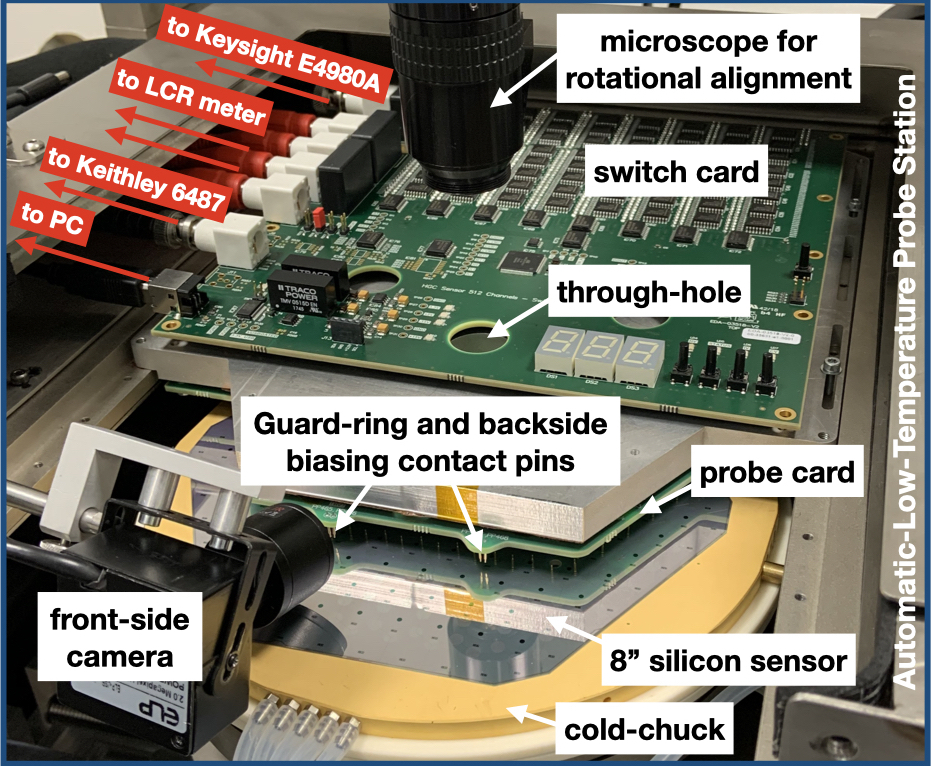
\includegraphics[width=0.75\textwidth]{figures/ALPS_photo_edit.jpeg}
	\caption{
		A low-density HGCAL silicon pad sensor right before connecting to the switch- and probe-card ARRAY system inside the Automatic-Low-Temperature-Probe Station (ALPS) at CERN.
		The probe station was closed and flushed with dry air during the testing to prevent the formation of ice.
		}
		\label{fig:ALPS_setup}
	\end{figure}
The silicon sensors were first placed on the chuck and then connected to the probe- and switch-card based ARRAY system~\cite{pitters:array2019}.
Through-holes in the cards and the probe station's microscope  enable sufficient sensor-to-pin alignment. 
The high voltage from the power supply was provided to the chuck and to the sensor's backside via dedicated pads on the sensor's front side.
Also the guard ring was accessible via a dedicated pad and could be connected with dedicated pins on the probe cards.
Two probe cards specific for the high- and for the low-density sensor layouts had been designed and manufactured for the tests.
The switch card was operated with a bias resistance (R$_\text{bias}$) of \SI{1}{\mega\ohm} and a high voltage resistance (R$_\text{HV}$) of \SI{12}{\kilo\ohm}, see Figure$~$9 in$~$\cite{pitters:array2019}.
In this configuration, the ARRAY system is designed to withstand total leakage currents up to \SI{2}{\milli\ampere} and per-pad currents up to \SI{10}{\micro\ampere}.
Since these limits would have been exceeded by a few orders of magnitude at room temperature, cooling the neutron-irradiated sensors down to \SI{-40}{\celsius} was imperative.
The spatial variation of the C200-40 chuck's temperature profile at this temperature amounts to $\pm\SI{0.5}{\celsius}$, cf.~\ref{appendix:chuck_temp}, whereas fluctuations with time are found to be negligible. 
For the purpose of preventing the formation of ice, the probe station had to be flushed with dry air. 
With total currents at the order of $\mathcal{O}(\SI{1}{\milli\ampere})$, the voltage drop at R$_\text{HV}$ for the testing of neutron-irradiated sensors was non-negligible and was corrected for.
The voltage at the silicon pad under test is referred to as "effective bias voltage" in this work.
Per-pad leakage currents were measured with a Keithley 6487 picoammeter, whereas total currents were measured directly with the Keithley 2410 power supply.
A Keysight E4980A LCR meter was operated at a frequency (f$_\text{LCR}$) of \SI{2}{\kilo\hertz} for the inference of the per-pad impedance.
This particular frequency was chosen to minimise the error associated to the capacitance that is derived from it~\cite{pitters:array2019}.
%It was found empirically that the impact on the end capacitance is negligible whereas the derived depletion voltages are increased by about \SI{10}{\percent} when reducing f$_\text{LCR}$ to \SI{500}{\hertz}. 

\subsection{Characterisation Procedure}
\label{subsec:setup_procedure}
After connecting the sensor to the probecard, per-pad leakage currents as a function of the bias voltage (IV) for all pads on a given sensor were measured first.
This was preceded by a per-pad capacitance vs. bias voltage assessment (CV).
After each iteration over all pads at a fixed bias voltage, voltages were incremented in varying steps between 50-\SI{100}{\volt} up to \SI{850}{\volt}, whereby the exact choice depended on the measurement type (IV/CV) and on the thickness of the tested sensor.
Although not applicable for the results shown in this work, it should be noted that a given measurement sequence was aborted if the total leakage current exceeded \SI{2}{\milli\ampere}.
Similarly, individual pads whose leakage currents exceeded \SI{5}{\micro\ampere} were not measured any further and in particular were excluded from the subsequent CV.
These compliance limits prohibited large voltage drops inside the test circuitry minimising the risk of harmful damage to the ARRAY system.
The entire characterisation sequence was fully automatised as a publicly available LabView-based program (HexDAQ version 1.5.1~\cite{labview_hexdaq}).
Including voltage ramps and settling times, IV measurements of low-density sensors took about \SI{1.5}{\hour} (CV: \SI{2.5}{\hour}), whereby the duration was about twice as long for high-density sensors.
In order to quantify the potential of sensor curation via beneficial annealing, silicon sensors were also warmed up to \SI{60}{\celsius} for a total of \SI{80}{\min}\footnote{Corresponding to about two weeks at room temperature.} inside the probe station.
IV and CV characterisations were conducted before and after additional annealing.